\documentclass[12pt, a4paper,titlepage,openany]{article}
\usepackage[italian]{babel}
\usepackage[T1]{fontenc}
\usepackage[table]{xcolor}
\usepackage{float}
\restylefloat{table,figure}
\usepackage{graphicx}	
\usepackage[utf8]{inputenc}
\usepackage{amsmath}
\usepackage{fancyhdr}
\pagestyle{fancy}
\cfoot{\thepage}
\renewcommand{\footrulewidth}{0.25pt}
\usepackage{amssymb}
\usepackage{amsthm}
\title{Dispensa di Machine Learning}
\author{Federico Luzzi}
\date{}

\begin{document}
	\maketitle
	
\tableofcontents
\section{Lezione 1}

\subsection{Introduzione}
Gli ambiti più importanti nei quali vengono applicate tecniche di machine learning nella vita reale sono:
\begin{itemize}
	\item Finanza
	\item Sanità
	\item Agricoltura
	\item e-commerce
	\item Social
	\item Chatbot
	\item Sensoristica (come i veicoli a guida autonoma)
\end{itemize}

Vista la grande mole di dati la necessità è capire come trattare i dati.
\textbf{L'obiettivo del Machine Learning è sviluppare metodologia per dare valore ai dati in funzione di una particolare domanda che ci stiamo facendo.}

Tipicamente si divide in tre macro categorie.
\begin{itemize}
	\item Apprendimento supervisionato o predittivo: qualcuno ha gia catalogato ad esempio delle immagini o dei dati e noi prendendo questi modelli dovremmo essere in grado di predire.
	\item Apprendimento descrittivo: ci sono delle funzioni obiettivo che vanno ottimizzate. Non usiamo etichette della singola istanza ma in qualche modo sappiamo dove arrivare.
	\item Apprendimento rinforzato: E' quello più utile in questa epoca: funziona sui premi.
\end{itemize}

In questo corso ci concentreremo sui primi due tipi di apprendimento.

\textit{L'apprendimento supervisionato} si divide a sua volta:
\begin{itemize}
	\item Classificazione: quando sono quantità discrete da dividere
	\item Regressione: con una data lettura cerco di prevedere dei dati.
\end{itemize}

\textit{L'apprendimento non supervisionato} si divide a sua volta:
\begin{itemize}
	\item Clustering: Vuol dire mettere ordine nelle istanze che ci vengono presentate.
	\item Associativa: Scopre pattern che descrivono bene caratteristiche associate ad un certo fenomeno.
\end{itemize}

Per alcuni compiti la correlazione va benissimo, in alcuni casi però addirittura ci danneggia. Se provassi a vedere la correlazione tra il numero di omicidi in america e il numero di fondi investiti sulla ricerca scientifica vedrei che statisticamente sono strettamente correlate. Questo è ovviamente un no-sense.

\textbf{Paradosso di Simpson:} Se uso solo i dati senza modello no c'è alcun modo di scoprire la verità


\subsection{Data Types}

Il primo passo fondamentale è sicuramente quello di prendere confidenza coi dati. E' fondamentale capire la natura dei dati che abbiamo a disposizione (\textbf{dataset}), c'è un fenomeno che si chiama \textbf{churn}, quando non siamo soddisfatti di un servizio ci affidiamo al competitor.

Ci possono essere valori missing in un dataset e possono mancare per diversi motivi.

Le colonne sono chiamate \textbf{Attributi.}

Le righe sono chiamate \textbf{Istanze.}

A volte ci sono anche attributi duplicati che possiamo tranquillamente buttare fuori.
Ogni attributo è caratterizzato dal fatto di avere un tipo. Conoscerlo è fondamentale per trattare i dati.
Gli attributi si dividono in due grandi gruppi:
\begin{itemize}
	\item Categorici:
	\begin{itemize}
		\item Nominali: ad esempio il colore degli occhi.
		\item Ordinali: ad esempio possono essere i giudizi.
	\end{itemize}
	\item Numerici:
	\begin{itemize}
		\item Intervallo: ammettono operazioni di somma e sottrazione. 
		\item Ratio: possiamo applicare tutte le operazioni logico/matematiche.
	\end{itemize}
\end{itemize}

Dall'alto al basso il livello gerarchico sale e le proprietà aumentano.

Si possono anche dividere in attributi \textit{discreti} che possono essere:
\begin{itemize}
	\item Categorici
	\item Numerici
	\item Binari: sono i più particolari da trattare, e hanno una serie di proprietà strane.
\end{itemize}
Oppure possono essere \textit{Continui.}

\subsection{Data exploration}

Dobbiamo però anche sapere come esplorare i dati. Per farlo facciamo cose molto elementari.
Per farlo si usano tutti gli strumenti a nostra disposizione.

Il concetto di \textbf{quantile} è trovare il numero di osservazione che ci indica quanti attributi sono più piccoli di un dato valore.
Un quantile molto importante è il quantile di ordine $\frac{1}{2}$ e si chiama \textbf{Mediana} che è quello che ha esattamente minori di lui la metà dei dati.

\[mean = \frac{1}{n}\sum_{i=1}^{n}x_i\]

La media non è un buon modo di visualizzare i dati perché dice poco ma quanto meno dice qualcosa. Siccome la media è basata su singole osservazioni si possono vedere le presenze di outliar, ossia di elementi troppo discordanti dalla media e che si presenta poche volte. Sono quindi elementi che è necessario trattare per vedere la provenienza.

Per prevenire questo si usa la \textbf{media trimmed} in cui si buttano via il valore più piccolo e il valore più grande. Se si trova un grosso scostamento probabilmente è presente un outlier.

Si puù definire anche il range anche se di solito si usa la varianza:
\[var = \frac{1}{n}\sum_{i = 1}^{n} (x_{i} - \bar{x})^{2}\]

Di solito si usa la deviazione standard che ha lo stesso ordine di grandezza dei dati:

\[ std = \sqrt{var} \]

Si usa anche il range interquartile (IQR) sempre per ovviare alla presenza di outliar.
Se ho a che fare con coppie di attributi allora è naturale parlare di \textbf{covarianza} ossia la varianza calcolata su due attributi diversi:

\[cov(X,Y) = \frac{1}{n}\sum_{i = 1}^{n} (x_{i} - \bar{x})(y_{i} - \bar{y})\]

Di solito si fanno scalature perché sennò le covarianze vengono troppo sbagliate. Per ovviare uso la \textbf{correlazione di Pearson} che può prendere valori $[-1,1]$
\[ corr(x,y) = \frac{cov(x,y)}{\sqrt{var(x)var(y)}}\]

Possono organizzare i dati in istogrammi in cui posso usare una ampiezza fissa o variabile (bin). A seconda dell'ampiezza che uso posso ottenere due disegni molto diversi.

Un altro modo di rappresentare i dati particolarmente utile è il \textbf{grafico Box and Whiskers} applicato solo ad attributi quantitativi.

\subsection{Missing replacement}

E' un problema enorme di per sè. Le operazioni più elementari sono le seguenti. In alcuni valori degli attributi un valore non è registrato. Ci possono esser tante ragioni: ad esempio un attributo non è sempre stato osservabile (penso all'ambito clinico), o ad esempio un attributo prima non veniva considerato rilevante.

Il primo nmetodo è il \textbf{Record removal} che è molto drastico come metodo perché comunque sia vengono eliminati dei valori che sarebbero potuti essere molto importanti.

Il secondo metodo è quello di \textbf{imputazione manuale}: è fatta da umani e tramite osservazioni ci si chiede se sia possibile inserirlo, è tremendamente difficile dal punto di vista computazionale.

Il terzo metodo è quello della \textbf{global constant}: ossia metto un numero là chiamato place holder con un valore costante, non troppo efficiente.

Il quarto metodo è quello di \textbf{rimpiazzarlo con la moda}, anche questo però è fortemente criticabile.
Se gli attributi sono continui si fa la stessa cosa ma con la media.

Il quinto metodo è \textbf{Conditional mean replacement} ossia bisogna rimpiazzare con la media solo se è presente un altro determinato attributo.

Il sesto metodo è quello del \textbf{most probable} ossia di prendere un modello e sostituire il valore.

E' molto difficile dare il confine tra l'esplorazione dei dati e la modellizzazione dei dati.

\subsection{Data Preprocessing}

Tutti questi processi impattano fortemente tutta l'analisi che farò dopo.
\section{Lezione 2}
Da fare
\section{Lezione 3}
\subsection{Classification}
Entriamo un po' più nella componente di validazione nei modelli di classificazione supervisionata.
La cosa più importante è \textbf{capire cosa stiamo facendo.}

In questa lezione parleremo di:
\begin{itemize}
	\item Variabile di classe
	\item Modellizzazione descrittiva
	\item Training set/ test set
	\item Modelli di classificazione
	\item Matrice di confusione
	\item Accuratezza
\end{itemize}

Nel solito dataset vogliamo capire quale sia la particolare combinazione di attributi che abbiamo che determini se un cliente abbandoni il nostro servizio o meno.
Bisogna prima vedere di che tipo siano le variabili presenti nel nostro database.

Dobbiamo essere in grado sia di prevederlo che di capire perché qualcuno ha abbandonato. Svolgiamo questo compito con un modello di \textbf{classificazione}. Un modello di classificazione è un modello che sfrutta alcuni attributi del dataset per prevedere un valore di un altro attributo.
Possiamo vederlo come:

una scatola che ha degli ingressi che \textit{sono gli attributi che usiamo per svolgere il nostro compito} e ha degli output che corrisponde alla \textit{variabile da categorizzare.}

Le variabili in input si chiamano \textbf{variabili esplicative o variabili di input.}

Le variabili in output si chiamano \textbf{variabili di classe o variabili di output.}

Un \textbf{modello di classificazione} è qualcosa che risolve un problema di classificazione:
\begin{itemize}
	\item Modello descrittivo: serve come strumento di spiegazione per distinguere tra oggetti di classi diverse
	\item Modello predittivo: predice la classe di un record sconosciuto, pu\`o essere visto come una \underline{scatola nera} che asssegna una label di una classe al record sconosciuto
\end{itemize}

La tecnica di classificazione o \textbf{classificatore} è un approccio sistematico per costruire un modello di classificazione su un dataset.

Prenderemo quindi un \textbf{training set} che consiste in dei record in cui tutti gli attributi sono noti.  Una volta addestrato (apprendimento e validazione) il nostro modello questo verrà valutato su un insieme di dati chiamato test set.

Il \textbf{test set} consiste in dei record le cui label di classe (o valori) sono sconosciute (o presunte tali).

Il modello che ne esce dal training con il training set si basa su un certo algorimo di apprendimento (\textbf{learner}), \`e questo la chiave di tutto.
\\
Io sono sempre interessato a ciò che deve predire più che a quelli che ho già.
Il training set è  quello principale su cui il modello impara da là passo alla feature selection perché mi accorgo che magari qualche attributo non è necessario nelle predizioni ma fa solo rumore. In particolare è l'algoritmo di apprendimento che dice come il modello impara. 

Il modello trainato si chiama \textbf{inducer}, in pratica un'istanza del modello di classificazione. All'inducer viene chiesto di predire il valore dell'attributo di classe per il test set.

Bisogna valutare ora le performance del modello inducer. Uno dei modi per analizzare se è venuto bene devo usare la \textbf{matrice di confusione.} Nelle righe vi sono i veri valori delle classi, nelle colonne i valori predetti dall'inducer. Il numero di righe è uguale al numero di colonne e corrispondono al numero di classi.

\begin{figure}[h!]
	\centering
	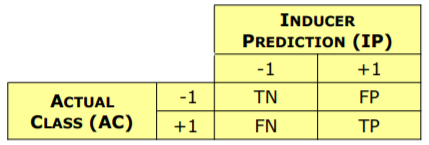
\includegraphics[height=0.2 \linewidth]{pict/matrconf.png}
	\caption{modello di matrice di confusione}
\end{figure}

Definiamo una misura che si chiama accuratezza:

\[accuracy = \frac{\sum_{i = 1}^{n} diagonal}{\sum_{i=1}^{n'}elements} = \frac{TN + TP}{TN + TP + FN + FP}\] 

La misura complementare che troveremo indicata è quella degli elementi:

\[error =  1 - accuracy\]

\subsection{Tecniche di classificazione}
Una tecnica di classificazione è un modo sistematico di aggredire un dataset, in particolare possiamo dividerle in 4 macro categorie:
\begin{itemize}
	\item Euristici: ispezionano il suo vicinato come (Decision Trees, Random Forest, Nearest Neighboor)
	\item Regression Based: usa la probabilità condizionata parametrica, regressione logica
	\item Separazione: partiziona lo spazio degli attributi, fa riferimento alle Support Vector Machine e alle Artificial Neural Network
	\item Probabilistici: usano la formula di Bayes (Naive Bayes ecc...) e si dimostra particolarmente efficiente.
\end{itemize}

Forniremo una overview di tutte queste, non le tratteremo nel dettaglio

\subsection{Euristici}

Un \textbf{albero di decisione} ha innanzitutto una rappresentazione grafica che ci consente di approcciarci con più propensione. Vi sono 2 elementi: nodi e archi. Il nodo rappresenta un sottoinsieme del dataset, gli archi sono usati per modellare gli output di modelli diversi di dataset.

\begin{figure}[h!]
	\centering
	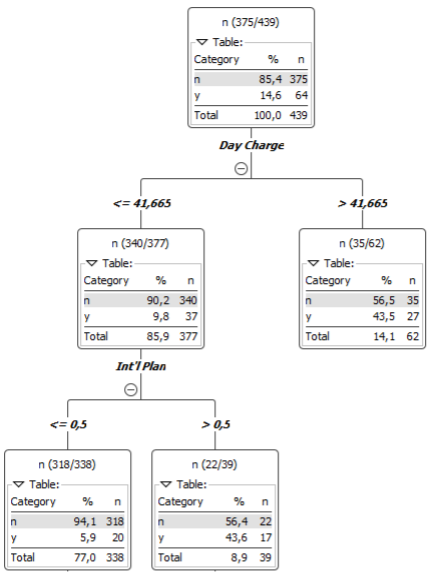
\includegraphics[height=0.7 \linewidth]{pict/decision_tree.png}
	\caption{modello decision tree}
\end{figure}

I suoi ingredienti pricnipali sono:
\begin{itemize}
	\item Nodo a radice: non ha archi in ingresso ma può averne più di due in uscita.
	\item Nodi interni: hanno un solo arco in ingresso e alemeno due in uscita.
	\item Nodi Foglia: sono nodi interni senza archi in uscita.
\end{itemize}
Cerchiamo di capire come si forma questo albero: ad ogni nodo è associato un determinato schema.

Subito dopo il primo nodo (radice) abbiamo l'indicazione di un attributo: ad esempio posso chiedermi se 'day charge' sia minore di 41 o maggiore e dividere l'albero in due nodi. Se la risposta è vero allora mi muovo in un nodo altrimenti nell'altro.

All'interno del nuovo nodo ho di nuovo la valutazione di una variabile, e proseguo cos\`i finch\`e raggiungo un nodo foglia.

Quando arriviamo ad una foglia devo fornire una risposta, ovvero conto la classe più frequente ed rispondo al chiamante con essa (es. churn = n).

Per la valutazione delle \textbf{performance} vengono utilizzati i seguenti indici: entropia, indice di Gini e il classification error. 

Inoltre va notato che il \textbf{tipo} di attributo utilizzabile pu\`o essere: binario, nominale o continuo.

E' un modello che risponde sempre la classe più frequente ed è un modello praticamente inutile quando ho delle classi particolarmente sbilanciate. Sono evidentemente test univariati, ciò che faccio è costruire iper parallelepipedi del nostro dataset.

Il risultato di queste rette fa la differenza sulla capacità di evidenziare dove ci siano elementi di una certa classe, devo quindi imparare a posizionare questi iperpiani: \textbf{Voglio partizionare il mio spazio in iperpiani massimizzando l'accuratezza.}

Non c'è alcuna ragione per cui io non possa usare degli splitting multipli e non solo su binari, posso farlo anche su valori nominali.

I segmenti degli iperpiani si chiamano \textbf{decision boundary} e sono quelle che passano dalle classi, il confine tra diverse aree della separazione delle classe. \`E un metodo computazionalmente dispendioso se ho molte variabili da valutare.

\subsection{Regressione Logistica Binomiale}

Servono per risolvere problemi di regressione binaria a diversi livelli. E' applicabile ad attributi continui e con certe accuratezze anche ad attributi nominali.

Si assume l'attributo di classe $Y = \{0,1\}$, allora il classificatore a regressione logistica binomiale calcola a posteriore la probabilit\`a che $Y$ assuma il valore di un input esplicativo $X$. Si cacola come segue:

\[P(Y = 0 | X= \bar{x}) = \frac{1}{1+e^{\bar{x}  \bar{w}}}\]

\[P(Y = 1 | X= \bar{x}) = \frac{e^{\bar{x}  \bar{w}}}{1+e^{\bar{x}  \bar{w}}}\]

dove $\bar{w}$ \`e chiamato il vettore parametro.

In questo modo vengono portate le probabilità di appartenere ad una certa classe.	

\section{Lezione 4}

\textbf{Cross-validazione}: quando facciamo l'apprendimento, se ci sono parametri per ottimizzare il modello è buona norma provare diverse combinazioni di parametri in fase di apprendimento. (detto informalmente)

\textbf{Random forest}: \`e un comitato di alberi di decisione. Sostanzialmente usa degli attributi che sono in generale sottoinsiemi degli attributi, ogni albero può avere un sottoinsieme differente di attributi. Ogni albero usa attributi in modo randomico. Ognumo apprende a modo suo e il random forest in base a dei parametri (regione dello spazio) decide a quale albero dare retta. 

\subsection{Support Vector Machines}
Metodi di classificazione con separazione. Lo scopo \`e separare o "apprendere" classi che vogliamo classificare. In uno spazio bidimensionale possiamo tracciare una retta (se ho due sole classi) per cui definisco l'area di appartenenza di una o dell'altra classe. La retta in questione è definita dalla seguente equazione:

$\bar{w} \cdot \bar{x} + b = w_1 x_1 + w_2 x_2 + b = 0$\\
per orientare la retta utiliziamo il vettore $\bar{w} = [w_1,w_2]$ oppure $b$. ($\bar{w}$ fa ruotare, $b$ fa traslare)\\
se la retta esiste allora l'insieme delle istanze è \underline{linearmente separabile}.

\textit{Problema}: vi sono pi\`u (anche infinite) rette utilizzabili per effettuare la separazione, quale devo scegliere? Perch\`e non basta trovare una retta che funziona, ma la retta migliore per quando si dovr\`a valutare dati nuovi. Si crea una sorta di area grigia nlla quale non so dire esattamente quale delle due classi categorizzare.

inserisci immagine slide 

devo sostanzialmente trovare una retta che \textbf{massimizza il margine di errore}. L'optimal linear decision boundary. 

inserisci altra immagine slide (dove vedo il margine di errore)

la retta $B_1$ è nettamente preferita rispetto alla retta $B_2$.

Naturalmente per n attributi bisogna trovare l'iperpiano ottimale per dividere un determinato insieme di istanze. Matematicamente parlando si cerca di massimizzare il margine $\delta = 1 / |w|^2$, la retta ha la seguente impostazione: $\bar{w} \cdot \bar{x} + b = 0$, le rette ai confini del margine sono fissate a $\bar{w} \cdot \bar{x} + b = 1$ e $\bar{w} \cdot \bar{x} + b = -1$. 

$h(\bar{x}) = $

L'argomento della retta \`e in 2 dimensioni, per\`o dopo aver applicato la funzione h(x) quella retta diventa un piano che va a -1 da un lato e a 1 dall'altro.

\[min \frac{1}{2}\bar{w} \cdot \bar{w}^T \]

Per trovare la retta devo minimizzare l'inverso del margine $\delta$\\
bisogna imporvi dei vincoli per ogni attributo, se $\bar{w}$ e $\bar{x}$ sono \textit{concordi in segno} (positivo o negativo) allora classifica perfettamente perch\`e il risultato è $>= 1$. Garantiscono che tutti i casi del dataset siano classificati correttamente e tra tutti i casi che classificano correttamente scelgo quello che massimizza il margine. 

Non risolveremo questa formula di ottimizzazione in modo diretto, ma la sua formulazione \textbf{duale}. In ogni caso questa formulazione funziona bene se il problema \`e \underline{linearmente separabile}.

Nei casi \textbf{non} linearmente separabili, non esiste \textbf{mai} una retta in grado di separare correttamente le classi. In questi casi la formulazione precedente non ammette soluzione, perch\'e per alcuni dati i vincoli non ammettono soluzione. 

Si introducono allora le \textbf{Linear Soft-margin}:

$min $

il chi deve essere non negativo (variabile di slack), se utilizzo questo parametro di una certa quantit\`a per ammettere un errore allora esiste almeno una retta che risolve il problema di ottimizzazione. Ho sostanzialmente \textit{rilassato} il problema di ottimizzazione, in particolare i vincoli. Graficamente parlando \`e come traslare degli elementi di una classe diversa dalla regione di appartenenza verso la regione della classe di quell'elemento.

NB: i vettori di supporto sono quelle osservazioni che sono sul bordo del margine

Altra soluzione fattibile \`e utilizzare una funzione \textbf{non lineare}. Si va a cercare una trasformazione che porti dallo spazio originale in uno spazio delle features in cui posso applicare una separazione lineare. Sono in grado di separare il nuovo dataset nello spazio delle features. In questo modo posso sfruttare tutta la metodologia precedente ma in uno spazio "controllato". 

la traslazione avviene attraverso una funzione $\phi$: $\bar{w} \cdot \phi(\bar{x}) + b = 0$. Il modello diventa:

$ min $ ...

per l'apprendimento utilizziamo sostanzialmente delle funzioni kernel: $K(\bar{u}, \bar{v}) = \phi(\bar{u}) \cdot \phi(\bar{v})$. Queste funzioni kernel sono delle funzioni di similarit\`a calcolate nello spazio attributi originale di $x$.

\subsection{Reti di neuroni artificiali}
Oggi si utilizzano molto per il deep learning.

Un modello \textbf{MLP Multi-layer perceptron} consiste in neuroni artificiali che comunicano in modo unidimensionale dall'input X alla variabile di classe (volendo ci possono essere pi\`u neuroni di ouput).

Dati 3 neuroni di parametri continui, vengono inseriti in un neurone 4 che calcola una funzione. Ogni input nel neurone ha associato in peso $w$.
Il neurone calcola una \underline{combinazione lineare} tra gli input ed il peso dato ad esso. 

$z_4 = w_{1,4} \cdot x_1 + w_{2,4} \cdot x_2 +w_{3,4} \cdot x_3$

$z_4 - \theta_4$ threshold di soglia applicato alla combinazione lineare

$f(z_4 - \theta_4)$ funzione di attivazione (o trasferimento) che restituisce il valore che lui trasferir\`a ad un altro neurone o strato con cui comunica. Storicamente le funzioni applicazione sono la tangente iperbolica e la funzione logistica (intervallo tra -1 e 1 e tra 0 e 1). Oggi vengono utilizzate delle funzioni non derivabili pi\`u complesse, come funzioni RELU (Retify Linear Unit) che assumono valore 0 nel semiasse negativo e 1 nel semiasse positivo.

Vi sono 3 tipi di neuroni: di input, di output e nascosti. Quelli di input comunicano con quelli nascosti (i cui valori non sono palesi a noi) e comunicano infine con quello/i di output. 

Ogni neurone di input \`e connesso con ogni neuroni di strato nascosto  ed ogni nodo di strato nascosto comunica con il nodo di output (rete fully-connected). Ogni arco ha associato un peso e ogni nodo ha un valore di soglia $\theta_j$ e una funzione di attivazione. 

Le scelte architetturali fanno la differenza nel risultato della computazione. Doppia scelta: quanti neuoni usiamo e quanti ne utilizziamo nello strato nascosto. Determina l'architettura della nostra rete. Posso pensare di aggiungere un \textbf{livello} di neuroni nascosti. Non vi sono teorie che dicono il numero di nodi e livelli di strati nascosti, si procede in modo empirico e si valuta il modello che funziona meglio. Non vi sono vincoli rispetto a comunicare saltando livelli. Non si pu\`o per\`o comunicare all'indietro, infatti queste reti sono chiamate \textbf{feed-forward neural network} (possono possedere fino a centinaia di strati nascosti).

Per migliorare l'apprendimento si pu\`o propagare le valutazioni fatte all'output per tutti i nodi risalendo fino all'input. Modificando i pesi degli archi. Questa cosa funziona bene e ha senso con le RELU.

Il problema MLP. non ha soluzione oggi, pertanto si procede in modo empirico, non \`e ancora possibile arrivare ad una soluzione ottima, non si riesce a capire se si ha raggiunto il massimo/minimo globale ma si cerca quella che da risultati accettabili e migliori di altri. 

NB: classificare non significa saper approssimare!! Le SVM sono cos\`i, non adatti a modellare la probabilit\`a.

\section{Lezione 5}

\textbf{Classificatori probabilistici} calcolano la probabilit\`a condizionata e cercano di capire il valore della classe attributo da altre variabili. Si basa sul \textbf{teorema di Bayes}. 

\[P(Y|\bar{X}) = \frac{P(\bar{X}|Y) \cdot P(Y)}{P(\bar{X})}\]

dove:
\begin{itemize}
	\item $P(Y)$ è la probabilit\`a della classe attributo
	\item $P(\bar{X}|Y)$ la verosimiglianza di un vettore di attributi data la classe attributo
	\item $P(\bar{X})$ probabilit\`a dell'evidenza (nel senso di certezza)
	\item $P(Y|\bar{X})$ probabilit\`a a posteriori della classe attributo dato il vettore di attributi esplicativi
\end{itemize}
\subsection{Naive bayes}
Supponiamo Y attributo di classe binario \{-1,+1\}, $\bar{X}$ \`e attributo esplicativo binario $\{male, female\}$

Sostanzialmente una volta che comprendo le probabilit\`a condizionate tra attributo di classe e attributi esplicativi, applico la formula di bayes per inferire la classe pi\`u probabile. 

Quando il numero di variabili esplicative cresce (n variabili), le devo \underline{binarizzare} quindi avr\`o $2^n$ parametri. Che raggiungendo $n=30$ si arriva a pi\`u di un miliardo di parametri, valore assolutamente inaccettabile.

Bisogna allora fare un'assunzione: dati X, Y, Z. Diremo che X \`e indipendente condizionatamente da Y dato Z, se e sono se la probabilit\`a di X è indipendente dal valore dell'attributo Y una volta che Z sia noto. 

$\forall i,j,k P(X=x_i|Y=y_j, Z=z_k) = P(X=x_i|Z=z_k)$

Se assumo questa espressione per le variabili utilizzate si riduce enormemente il numero di parametri da computare, ci permette di andare da $2^n$ a $2 \cdot n$, in quanto $P(X_1, ..., X_n|Y) = \prod_{i=1}^n P(X_i|Y)$

Il record di variabili viene etichettato con il valore di classe che massimizza la probabilit\`a a posteriori.
La probabilit\`a computata a posteriori \`e:

\[P(Y=y_k|X_1,...,X_n) = \frac{P(Y=y_k)\cdot \prod_{i=1}^{n}P(X_i|Y=y_k)}{\sum_{j}P(Y=y_j) \cdot \prod_{i=1}^{n}P(X_i|Y=y_j)} \]

Naive Bayes fa parte dei modelli \textbf{grafico-probabilistici}. Un intera famiglia di modelli di questo tipo: reti bayesiane dinamiche, ecc... non andremo nel dettaglio.

\begin{figure}[h!]
	\centering
	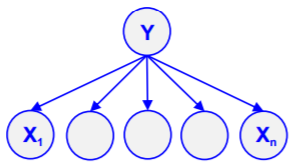
\includegraphics[height=0.3 \linewidth]{pict/naivebayes.png}
	\caption{rete naive bayes}
\end{figure}

A fianco del risultato output comunque \`e bene fornire la probabilit\`a con il quale si \`e ottenuto il risultato, in modo da dare una \textit{misura di affidabilit\`a}. 

il Naive bayes pu\`o essere applicato a attributi numerici quali intervalli e ratio. Ogni attributo numerico è associato a una densit\`a di probabilit\`a condizionale di classe normale. 

Solitamente si combinano attributi categorici (nominali e ordinali) con attributi numerici. 

Naive bayes si comporta generalmente bene ma richiede \underline{una enorme premessa} per essere applicato correttamente (\textbf{indipendenza condizionata}). Quindi \`e stata creata una versione pi\`u flessibile mantenendo la stessa capacit\`a computazionale.

\subsection{Reti bayesiane}
Una rete Naive bayes \`e generalizzata dalla \textbf{rete bayesiana} che \`e meno forzata dall'assunzione di indipendenza condizionata. 

\begin{figure}[h!]
	\centering
	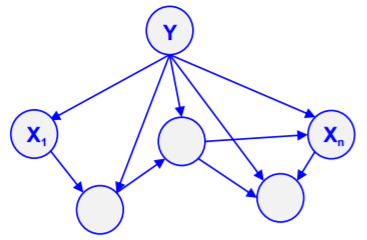
\includegraphics[height=0.35 \linewidth]{pict/networkbayes.png}
	\caption{rete bayesiana generalizzata}
\end{figure}

In queste reti vi \`e sempre il nodo radice Y che corrisponde all'attributo di classe, ma anche \underline{gli attributi esplicativi possono puntare ad altri attributi esplicativi}. Inoltre va notato che nel grafo \textbf{non} vi possono essere cicli in quanto un nodo successivo non pu\`o essere causa di un nodo precedente. Per ogni nodo va specificata una tabella di probabilit\`a condizionata rispetto al valore dei suoi genitori. In sostanza prendo in considerazione tutte le possibili configurazioni dei genitori e per ognuna do un risultato figlio diverso.

Questo /`e un modello particolare di rete bayesiana che viene utilizzata per la classificazione. La cosa bella di questo modello \`e che anche con valori null si potr/`a comunque fare inferenza perch/`e nativamente ha questa caratteristica. 

Se io ti offro di valutare un certo attributo perch\`e sapendo il valre di quel attributo so che \`e condizionato da quell'altro che ho gi\`a calcolato.  

Nelle reti neurali \textbf{non} \`e possibile far computare un modello senza che io abbia tutti gli input. 

\subsection{Tree-augmented Naive Bayes}
\textbf{Tree-augmented Naive Bayes} oltre ad avere il nodo genitore Y pu\`o permettersi di avere un altro nodo genitore (sempre). Se io addestro la rete senza nodo di classe allora ho un albero, dopo inserendovi il nodo Y fa inferenza. 

\begin{figure}[h!]
	\centering
	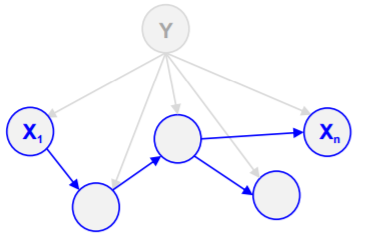
\includegraphics[height=0.35 \linewidth]{pict/treenaivebayes.png}
	\caption{tree-augmented Naive bayes}
\end{figure}

\`E molto potente per la feature selection, ovvero per la ricerca delle feature pi\`u significative. 

Ci sono altre modifiche possibili al Tree-augmente naive bayes, presenti il letteratura. 
\clearpage
\subsection{Summary}
Per capire come \textit{nativamente} si differenziano i modelli di classificazione vedi tabella successiva. 

\begin{figure}[h!]
	\centering
	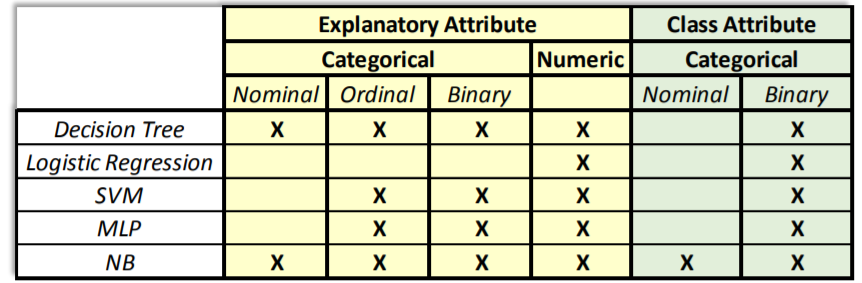
\includegraphics[height=0.3 \linewidth]{pict/class_tecniques.png}
	\caption{comparazione tra i principali modelli}
\end{figure}

\section{Lezione 6}

Abbiamo parlato di diversi tipi di modelli di classificazione con l'intento di prendere coscienza quali sono i parametri su cui si fondano questi modelli.
Ora dobbiamo mettere insieme il problema di mettere insieme questi modelli che abbiamo provato:

Stimare l'accuratezza di un modello non è efficace, quindi usiamo come stima quella che calcoliamo quella su un altro modello che è quello di test.

Ricordiamoci che se spingiamo troppo l'acceleratore andiamo in contro al modello di \textbf{overfitting} se invece stiamo troppo cauti allora andiamo in contro a problemi di \textbf{underfitting.}

Dobbiamo introdurre due grandezze:
\begin{itemize}
	\item Training error: E' un errore che commettiamo sul training set.
	\item Generalization error: è qualcosa la cui stima può essere ricavata da una stima sul test set ed è trattato come una variabile aleatoria.
\end{itemize}

Devo osservare se ci sono delle osservazioni replicate perché ciò infleunza fortemente l'accuratezza.

\underline{Un buon modello di training deve avere entrambi gli errori bassi.}


Un modello che si adatta molto bene all'errore sul training set ma che ha un errore molto grande sul test set è un modello che overfitta.

Dobbiamo avere quindi un buon compromesso che funzioni bene sia sul training set che sul test set. 

E' possibile anche il fenomeno contrario, quindi fare un modello troppo semplice che usa il test set come unico modello di interesse, questo fenomeno si chiama \textbf{under fitting}, in questo caso essa andrà male sia sul trainig che sul test. 

 Devo avere entrambi gli errori con un valore basso e  con valori vicini.
 
 Ricordiamo che l'erorre di generalizzazione non lo conosciamo ma faremo una stima con i dati di test. 
 Il modello ottimale sul training set non è quasi mai il migliore da applicare.
 
 
Vediamo ora che strumenti abbiamo a disposizione per evitare questo tipo di problema. E' fondamentale non limitarci all'accuratezza come  misura di performance di un algoritmo di classificazione.

Un altro limite è la \textit{velocità}, devo quindi usare un modello meno accurato ma che risponda meglio alle caratteristiche.

Vogliamo sviluppare un modello che ci garantisca la miglior prestazione possibile su dei nuovi dati. Questi modelli son spiegati su queste caratteristiche:
\begin{itemize}
	\item Accuratezza.
	\item Velocità.
	\item Robustezza.
	\item Interpretabilità.
\end{itemize}

\subsection{Accuratezza}

Misura la capacità del nostro modello di fornire buone predizioni sui dei nuovi records. Permette di selezionare l'istanza del modello in grado di garantire la migliore prestazione.

Usiamo la seguente notazione:

\begin{itemize}
	\item $D_{t}$: training set che consiste di t records.
	\item $D_{ts}$: test set che contiene s records.
\end{itemize}

Un buon indicatore della accuratezza è quello che usiamo sui dati di test.


\[L(y_{i}, f(x_{i})) =
\begin{cases}
	0 \quad se \quad  y_{i} = f(x_{i})
	\\ 1 \quad se \quad  y_{i} \neq f(x_{i})
\end{cases}
\]
Mi dice che gli errori sono tutti distribuiti allo stesso modo.

Calcolo l'accuratezza come:

\[ acc(D_{ts}) = 1 - \frac{1}{v} \sum_{i=1}^{v} L(y_{i}, f(x_{i})) \]

\subsection{Velocità}

Prima accezione della velocità è l'accezione del tempo che è necessario per apprendere un modello, questa variabile si è però un po' stemperata perché disponiamo di calcolatori molto molto veloci.

Lo spazio di memoria può essere un ulteriore problema, questo perché ci sono algoritmi che per imparare hanno bisogno di tenere tutto il dataset in memoria in ogni momento.

Se ci rendiamo conto che non riusciamo in termine di memoria a fare questo possiamo eseguire un \textbf{campionamento} per aumentare la velocità riducendo la memoria senza rinunciare ad una buona stima dei parametri. Questo però non entra quasi mai in gioco perché a meno di situazioni estreme non abbiamo problemi (fisici a LHC)

\subsection{Robustezza, Scalabilità e Interpretabilità}

Quando si parla di robustezza possono esserci:

\begin{itemize}
	\item outliers: sono talmente impattanti che possono rendere inutile l'apprendimento. E' importante verificare se ci sono queste informazioni completamente anomale.
	\item Missing data: sono reali e dobbiamo riconoscere che non possiamo misurare tutto e che i dati possono essere sporchi.
	\item Variazioni del training set e del test set: tutto il lavoro di sviluppo che stiamo facenod parte dal presupposto che dati di trainig e di test siano quanto meno simili, se questo viene a cadere allora tutto quello che abbiamo fatto è inutile. Questo fenomeno si chiama \textbf{concept stream.}
\end{itemize}

La \textbf{scalabilità} riguarda la capacità di imparare sempre di più man mano che aumento il numero di records. Le reti Bayesiane non lo sono per niente infatti funzionano bene solo con pochi dati.

L' \textbf{interpretabilità} è molto più complessa da descrivere. Il modo in cui gli umani imparano è tutto fuorché quantitativa. Questo perché noi siamo molto opiù bravi a ragionare per termini qualitativi. A seconda della persona con cui sto parlando devo cambiare il meccanismo con cui fornisco una spiegazione. Questo perchè se non uso il meccanismo giusto allora la spiegazione viene rifiutata. Una spiegazione deve far leva su pochi elementi ed usare un elemento comune per convincerlo.

\subsection{Hold out}

L'accuratezza è l'unica parte quantitativa che siamo in grado di calcolare.
Vediamo quali strumenti abbiamo a dispozione per stimare l'accuratezza. L'holdout consiste nel lasciare fuori una porzione dell'insieme di dati che abbiamo, si usa generalmente la regola:

\begin{itemize}
	\item Training set: $\frac{2}{3} dataset$
	\item Test set: $\frac{1}{3} dataset$
\end{itemize}

Immaginiamo di avere il nostro dataset D, prendiamo il training set $D_{t}$ che genera un inducer, forniamo il test set $D_{ts}$ all'inducer che calcola la stima. La stima dipende dalla scelta che noi facciamo per dividere il dataset.

Per immunizzarmi dalla sfortuna della scelta basta ripetere in modo iterato lo stesso processo.

\[D_{ts_{r}} = D - D{t_{r}}\]

Conduco in questo caso $r$ fasi di apprendimento, questo ovviamente ha un costo che pago per avere una stima più attendibile.
Potrebbe anche succedere che una specifica osservazione cada sempre nei casi di training e non nel caso di test, questo può essere un forte bias, soprattutto se questo è un outlier.

Per ovviare a questo problema si usa la \textbf{cross validation}. 

\subsection{Cross Validation}

Si prende l'insieme di dati, si fissa il numero \textbf{k} che identifica il numero di insieme che voglio creare.

\begin{itemize}
	\item Devono essere mutualmente esclusivi.
	\item La loro unione deve fornire tutto il dataset.
\end{itemize}

Non esiste un solo modo di formare quei k sottoinsiemi. Noi svolgeremo k fasi di apprendimento che verrà testata su ognuno di questi fogli k. A questo punto escludo ogni foglio $D_{k}$ che userò come dataset di test.

\underline{In questo modo ogni istanza entra ogni volta nell'insieme di test.}

Se ci sono doppioni questo discorso non è più garantito,.
\textit{A questo punto la media delle accuratezze è la nuova accuratezza.} Questo posso farlo perché i k insieme hanno approssimativamente la stessa cardinalità.

\[ acc = \frac{1}{K}\sum_{k = 1}^{K} acc(D_{k})\]

Fare una \textbf{k folds cross validation} lo si fa con pochi attributi e i valori di k sono 3,5,10.

La forma più estrema è la \textbf{LOOCV} in cui ogni records corrisponde ad un foglio k.

Tipicamente tutte le partizioni dovrebbero contenere la stessa proporzione (\textbf{Stratified sampling}.)


\section{Lezione 10}
\subsection{Classificazione non binaria}

Nella realtà sono i problemi che si trovano più spesso. Per farlo trasformiamo questo problema in tanti problemi da due classi. Possiamo farlo perché sappiamo che la classe giusta è una e una sola (multi class). Possono anche essercene più di una (multi label)

Questo schema di classificazione in cui si fanno tutte sotto classi binarie si chiama \textbf{Uno contro tutti.}

\section{Lezione 11}
\subsection{Prossimità}

Influenza in modo pesante la nostra soluzione di un nostro problema di clustering. Bisogna fare una scelta della misura con cui approssimiamo quanto sono simili gli elementi appartenenti allo stesso cluster.

Stiamo in larga parte determinando il successo o l'insuccesso di una tecnica di clustering.

\textbf{La analisi dei cluster affonda le sue radici nel concetto di cosa sia simile e cosa sia dissimile,} quando cerchiamo di esprimerlo in termini formali diventa abbastanza difficili.

La similarità dipende dalla caratteristica che voglio valutare. Possiamo però essere d'accordo sul dire che cerchiamo alti valori di similarità.

In generale la similarità è nulla se i due oggetti sono totalmente differenti sotto la caratteristica che stiamo vlautando ed è uguale a 1 se sono completamente uguali. Useremo il termine \textbf{proximity} per indicare sia la similarità che la dissimilarità. 

Non c'è ortogonalità tra la scelta della misura e l'esito che otterrò.

\[ s.d = [0, 1]   \qquad s =  1-d\]

Ci sono diversi problemi che nascono quando trasformiamo una similarità in dissimilarità e viceversa. Per gfarlo devo usare una trasformazione non-lineare. Posso usare però una cosa del genere:

\[ d' = \frac{d}{1+d}\]

Devo essere pronto a capire quale sia l'effetto che induco sul clustering che voglio valutare. Quello che succede è che sto comprimendo in modo più efficienti i valori che ho. Devo accettare di distorcere il mio intervallo di similarità, molte volte questa non è una cosa negativa. Devo valutare nella nuova scala il livello di similarità.

\textit{E' evidente quindi che la prossimità che esiste tra due record è funzione della prossimità tra i corrispondenti attributi dei due records.}

Chiariamo ora come calcolare la similarità nel caso che ci sia un singolo attributo. Ci sono diversi modi per farlo, la tabella è in figura.

Con gli attributi nominali non è così facile. Per risolvere questo problema si usa trasformarli in numeri. Cio si porta dietro un problema, il fatto è che sto considerando un intervallo come equidistribuito.

Ci sono diverse misure che si possono usare per la prossimità, ora ne andiamo a valutare alcune.

\subsection{Minkowscky distance}

Si usano quando gli attributi sono numericied è valutata nel seguente modo:
\[d(x,y) = \sqrt[r]{\sum_{k = 1}^{n}|x_{k}-y_{k}|^{r}}\]

\begin{itemize}
	\item Se $r = 1$ distanza di manhattan
	\item Se $r = 2$ distanza euclidea
	\item Posso farne anche il limite per r che tende a $\infty$
\end{itemize}

Deve essere:
\begin{itemize}
	\item Non negativa
	\item Simmetrica
	\item Disuguaglianza triangolare
\end{itemize}

Se valgono queste proprietà allora si parla di metrica, generalmente quelle che useremo per la prossimità non viene soddisfatta la disuguaglianza triangolare.
 Vediamo ora le prime misure di prossimità:
 
 \[ SMC(x,y) = \frac{n_{matching}}{n_{attributes}} = \frac{f_{11}+ f_{00}}{f_{11}+ f_{00} + f_{01}+ f_{10}}\]
 
 Questo è scomodo se non possiamo affermare se gli 0 siano veramente degli 0 (persona ha visto il servizio e non l'ha comprato oppure non ha visto il servizio e non può averlo comprato?), per il valore 1 invece è chiaro. In qeusto caso si utilizza un'altra misura che è derivata da questa misura, ossia si usa l'osservazione che gli 1 non siano a pari degli 0. Si definisce quindi il \textbf{coefficiente di Jaccard}
 
  \[ J(x,y) = \frac{n_{matching}}{n_{attributesexcept00}} = \frac{f_{11}}{f_{11}+ f_{01}+ f_{10}}\]
  
 La misura di Jaccard è distorta in funzione di pesare gli 1 come più pesanti. Se sono binari e simmetrici allora uso SMC qualora questo non valga allora uso J.
 
 Posso estendere ancora il coefficiente di Jaccard al \textbf{Tanimoto coefficient.}
 Questa misura è distorta per trattare dati sparsi, quindi tanti elementi in cui ho 0 e solo poche diverse da 0, questo si usa ad esempio nell'analisi del linguaggio naturale.
 
 \[ EJ(x,y) = \frac{x \cdot y }{||x|| ^{2}+||y|| ^{2} -x \cdot y  } \]
 
 Penso ai tweet, una parola che non c'è è più importante di una in cui non c'è.
 
 Proseguiamo ora con la \textbf{cosine similarity.}
 Viene usata quando tutti gli attributi sono di natura numerica, e si ignorano i match di natura 00.
 
  \[ cos(x,y) = \frac{x \cdot y }{||x|| \cdot ||y||  } \]
  
  Per quanto riguarda la \textbf{correlazione} si usa quella di Pearson:
  \[ corr(x,y) = \frac{cov(x,y)}{stdv(x)stdv(y)}\]
  
 Anche questa è ovviamente da usare solo con attirbuti numerici.
 
 Poniamoci tre questioni fondamentali:
 \begin{itemize}
 	\item Come trattare attributi che assumano scale di valori di ampiezza diversa, e cosa fare se sono correlati?
 	\item Come si calcola prossimità di record composti da diversi tipi di attributi?
 	\item Come calcolare la prossimità quando assegniamo una diversa rilveanza agli attributi specifici?
 \end{itemize}
Per risolvere il primo problema faccio la seguente cosa: posso normalizzare i valori, se non lo facciamo quando calcolo le distanze esse risultano totalmente distorte. L'altro problema è se gli attributi sono fortemente correlati, per correggere questo fatto dobbiamo pensare che la similarità sia il grado di correlazione che assumono questi attributi, per farlo si usa la distanza di Mahal:

\[Mahal(x,y) = (x- y)\Sigma^{-1}(x- y)^{T}\]

Se sono composti da differenti tipi di attributi allora per ogni attributo valuto tutte le misure fatte in precedenza, dopo averlo fatto allora uso una varibile indicatrice $\delta_{k}$. Una volta trovato allora la similarità è una media delle similarità dei singoli attributi.

\[similarity(x,y) = \frac{\sum_{k = 1}^{n}\delta_{k} s_{k}}{\sum_{k = 1}^{n}\delta_{k}}\]

E' molto complesso sostenere tutta questa specificità.

Se abbiamo a che fare con dati densi e continui allora di solito le distanze metriche vengono ad essere una buona rappresentazione, se i dati sono sparsi e asimettrici allora la scelta prevalente è quella di escludere gli elementi che sono basati sul conteggio delle concorrenze (Jaccard).

\subsection{Algoritmi di clustering}

Presentiamo a questo punto qualche algoritmo di clustering. Partiamo da uno degli algortitmi più diffusi: \textbf{algoritmo delle k-medie}, è basato sull'assunzione che esista un rappresentante per ogni cluster in grado di descrivere bene tutte le caratteristiche del cluster. Si basa tutto sul concetto di centroide.

Nel caso del clustering basato sul prototipo è dire se un'osservazione appartiene o meno ad un determinato cluster è dire quanto è simile o dissimile al \textbf{prototipo} della suddetta classe.

Ci sono diversi tipi di algoritmi basati sul prototipo e dipendono da diverse caratteristiche:
\begin{itemize}
	\item Ogni oggetto deve appartenere ad un singolo cluster.
	\item Ogni record è nella condizione di appartenere a più di un gruppo contemporaneamente.
	\item Se il concetto di cluster lo modelliziamo con una distribuzione di tipo probabilistico.
\end{itemize}

L'algoritmo delle k-medie è molto potente però si basa su ipotesi molto forti. Il prototipo in questo caso si chiama \textbf{centroide.} Per calcolarlo si calcola le medie tra massimi e minimi sia in orizzontale che in verticale, e il punto con quelle coordinate è il centroide. Qua l'assunzione è che io so già la divisione in cluster, scegliere il centroide in principio può fare una grande differenza sul clustering.

Bisogna scegliere un k adeguato al problema che stiamo svolgendo, a questo punto ciò che si fa è:

\begin{itemize}
	\item Scegliere per $k = 0$ quali sono i centroidi.
	\item Fare in modo che non si "pestino i piedi".
	\item Ripetere queste cose:
	\begin{itemize}
		\item Formo k cluster in modo da assegnare ad ogni record il suo centroide più vicino. E' ovviamente un meccanismo esclusivo.
		\item Calcolo il nuovo centroide per ogni cluster .
		\item Mi fermo fino a quando il centroide non cambia più.		 
	\end{itemize}


\end{itemize}

\section{Lezione 14- Cluster validity}	

La trattazione è sempre la solita, quindi abbiamo un problema di clustering da risolvere. Sappiamo che il risultato dipende sicuramente dalla misura della similarità che decidiamo di usare, se decidiamo che ci possano essere overlapping, e se possiamo ammettere che alcune osservazioni non si adattino bene per essere raggruppate.

Decidiamo quindi di impostare un piano sperimentale, quindi selezioniamo un certo numero di clustering e provarli per vedere quale funzioni meglio. Vorremmo avere quindi gli stessi metodi dei classificatori per capire quando un classificatore è meglio di un altro. Purtroppo il concetto di clustering è molto più complesso. Quando introduco un colore in un diagramma ho sempre una distorsione visiva che mi induce a non essere più oggettivo.

Per prima cosa bisogna sempre vedere se valgono le ipotesi di clusterizzazione:

\textbf{I dati si organizzano in qualche modo? La struttura organizzativa esiste sempre?}

Abbiamo indici \textit{esterni o supervisionati:} ci dice se i cluster condividono una caratteristica che non era stata comunicata a livello dei cluster.

Possono esserci anche gli indici interni: misurano la bontà di un algoritmo di clustering senza tenere conto delle informazioni esterne.

Abbiamo anche gli indici relativi che mi dicono qual è il numero ottimale di gruppi che devo formare.

\subsection{Indici esterni}

Pensiamo di avere un partizionamento $P = \{P_{1}, ..., P_{R}\}$ di R insiemi disgiunti con $m$ elementi. 

Vediamo ora la seguente cosa: $C = \{C_{1}, ..., C_{K}\}$, moi compariamo ora P con C per vedere 	quali siano i casi che si realizzano.
Ci sono ovviamente quattro casi che corrispondono agli indici esterni o supervisionate:

\begin{itemize}
	\item x e y appartengono allo stesso cluster sia per C che per P
	\item x e y appartengono allo stesso cluster per C ma non per P
	\item x e y appartengono a diversi cluster per C ma allo stesso per P
	\item x e y non appartengono allo stesso cluster nè per P nè per C
\end{itemize}

Ovviamente le coppie che possiamo formare sono:

\[M =  \frac{m(m-1)}{2} =  a+b+c+d\]

Valutiamo la accuratezza con l'indice di Rand:

\[R = \frac{a + d}{M}\]

Ovviamente riguarda gli elementi della diagonale che portano fuori strada, allo stesso modo dell'altra volta definiamo l'indice di Jaccard:

\[ J = \frac{a}{a+b+c}\]

Ci sono diverse misure \textbf{Da non ricordare ma da inserire.}

\subsection{Indici interni}

Prendiamo un insieme di clustering e valutiamo la validità come una media delle validità:

\[ overall \quad validity = \sum_{i = 1}^{K}w_{i} \cdot validity(C_{i})\]

Possiamo definire la \textbf{coesione} di un cluster come la somma dei pesi dei link nel grafo di prossimità che abbiamo formato per gli elementi appartenenti allo stesso cluster.

\[cohesion(C_{i}) = \sum_{x,y \in C_{i}}proximity(x,y) = \sum_{x,y \in C_{i} }similarity(x,y)   \]

Se consideriamo lo spazio degli attributi allora posso affermare che la coesione è direttamente proporzionale alla similarita.

Possiamo invece definire la \textbf{separazione} nel seguente modo:

\[separation(C_{i}, C_{j}) = \sum_{x \in C_{i},y\in C_{j} }proximity(x,y) = \sum_{x \in C_{i},y\in C_{j} }similarity(x,y)   \]

Se dividessi per il numero di elementi otterrei qualcosa di molto vicino all'average linkage.
Si può fare anche la stessa cosa sui prototipi facendo la stessa cosa calcolando la prossimità sui centroidi o sui medoidi a seconda dell'algoritmo che andiamo ad implementare.

Anche la separazione viene calcolata allo stesso modo, come facilmente intuibile però è un'operazione molto meno costosa rispetto a quella precedente.

C'è un altro modo ancora per valutare la separazione tra due cluster, calcolando quanto disterebbero se mettessi tutti i dati insieme con un centroide unico.

Devo vedere quali sono le scelte che devo fare per dare un peso al cluster.

Tutto quello che abbiamo visto valuta i cluster nel suo insieme, ci sono anche modi per valutare la qualità del singolo cluster, questo lo facciamo utilizzando diversi approcci.

Posso notare che magari unnendo o separando due cluster ottengo delle soluzioni migliori. Definisco quindi una misura che valuta quanto è buona l'assegnazione di un record ad un certo cluster.
Questa si chiama \textbf{misura di silhouette:}

\[s_{i} = \frac{b_{i}- a_{i}}{\max(a_{i},b_{i})}\]

Dove:
\begin{itemize}
	\item $a_{i}$ è la distanza media dell'oggetto i-esimo rispetto a tutti gli oggetti del cluster a cui appartiene.
	\item $b_{i}$ è il minimo delle distanze medie dell'oggetto i-esimo da tutti gli oggetti degli altri cluster.
\end{itemize}
LA domanda implicita è quindi: se non l'avessi messo in quel cluster ma nel cluster che rende $b_{i}$ minimo allora cosa cambierebbe? Noi vogliamo che ogni osservazione abbia un coefficiente di silhouette più vicino possibile a 1, se ha un coefficiente negativo ciò vuol dire che probabilmente ho sbagliato a inserire un'osservazione nel cluster.

In modo analogo posso calcolare l'indice per un insieme di valori di cluster.

L'ultimo elemento che riguarda le misure interne riguarda il \textbf{cophenetic correlation coefficient}, in questo caso la descrizione matematica è molto complessa. Si va a valutare quanto sia in accordo la matrice delle prossimità con la matrice cofenetica. Se la correlazione tra le due matrici è alta alloira quello che ha fatto il nostro algoritmo è buono.

\subsection{Paradigma di validità }

Vediamo come sia possibile per certi problemi muoversi in modo da far finta di sapere come sia fatto il mondo e vedere se le nostre previsioni sia corretta.

Decidiamo quale sia l'indice di validazione che vogliamo usare e a questo punto definiamo una ipotesi nulla di \textit{nessuna struttura.} Il tipo di ipotesi che si va a fare dipende dal tipo di problema, può essere ad esempio :
\begin{itemize}
	\item \textit{Random Position} (i records si distribuiscono casualmente nello spazio n-dimensionale dei record.)
	\item \textit{Random Graph } non mi interessa la posizione ma che ci sia una certa struttura di similarità.
	\item \textit{Random Label}: etichettare le osservazioni in modi differenti non cambia il tipo di coerenza che ottengo nel mio esperimento.
\end{itemize}

Queste sono le ipotesi nulle che si usano più spesso. A questo punto facciamo il test di ipotesi usando una \textbf{Analisi Monte Carlo e Bootstrapping.} Se ottengo valori che non sono così differenti dalla pura distribuzione casuale allora posso concludere che verosimilmente i dati non presentano nessuna struttura. A questo punto posso calcolare gli indici esterni/interni e vedere cosa succede.

Vogliamo sempre ottenere l'esito che l'ipotesi nulla venga rigettata.

\section{Lezione 15- Association}
\subsection{Introduzione}

Dovrebbbe essere il primo gradino della scala di cui parlavamo all'inizio delle lezioni. Tutto quello che abbiamo visto fa riferimento a formulare e rispondere a domande che stanno sul primo gradino della scala: se osservo che una variabile assume un certo valore cosa posso dire delle altre variabili?  A questa domanda devo immaginare di poter rispondere senza interagire col sistema. Ci permettono di rispondere a queste domande in tantissimi ambiti. Parleremo quindi di \textbf{Analisi associativa.}

E' molto utile in ambiti di marketing, sopratutto per l'ambito di cross-selling, ossia cose che solitamente vengono comprate insieme.

Ha il seguente obiettivo: \textit{Identificare quali siano gli item associati.}

Quello che noi forniamo infine sono regole associative o \textit{frequent item.} 

\subsection{Nomenclatura}
Cerchiamo ora una trattazione più formale e quantitativa del problema, per farlo non conteremo la molteplicità di un item all'interno del dataset (non ci interessa che ci siano 3 o 4 confezioni di formaggio) ma ci interessa una trattazione binaria (il formaggio c'è o non c'è?)


Organizziamo il nostro dataset come un database relazionale, quindi organizzato in colonne (che corrispondono ai diversi item) e in righe (che corrispondono alle diverse transazioni).

Sia $I = \{i_{1}, i_{2}, ..., i_{d}\}$ l'insieme di  item in cui ovviamente non ci sono ripetizioni, supponiamo ora di avere anche l'insieme delle transazioni, $T = \{t_{1}, t_{2}, ..., t_{n}\}$ 
Supponiamo ora di prendere in considerazione una certa transazione, e di trovare una certa distribuzione di item in quella transazione, se un insieme contiene $k$ item allora viene chiamato \textit{k-itemset}, possono esserci anche insiemi vuoti (come transazioni in cui non viene comorato nulla.)  I k-itemset sono quindi sottoinsiemi di una transazione. Si dice che una transazione contiene un itemset se quest'ultimo è un sottoinisieme dell'itemset totale. C'è quindi una forte natura combinatoria e probabilistica insita nel problema.

Vado a contare quindi quante volte un dato itemset si presenta all'interno delle transazioni: questo conteggio si chiama \textit{support count.}


\[ \sigma (x)  = |\{\}|\]

Possiamo quindi definire le \textbf{regole associative:}

\[X  \implies Y\]
Dove X e Y sono due insiemi disgiunti.

Il \textbf{Supporto} determina quanto spesso una regola è applicabile ad un certo dataset.

\[s(X  \implies Y) =  \frac{\sigma(X \cup Y)}{N}\]

La \textbf{confidenza} è qualcosa che sconta l'assunzione del vero per quanto riguarda l'antecedente, qua si vede la forte asimmetria del problema.

\[s(X  \implies Y) =  \frac{\sigma(X \cup Y)}{\sigma(X)}\]

E' molto importante il supporto perché ci dà delle regole per decidere se vale  o meno la pena di guardare una certa regola di associazione.  Più alta è la confidenza più è vero che il conseguente si presenti data la presenza dell'antecedente.

Il \textbf{problema della ricerca delle regole associative}: dato un insieme di transaziooni, fissiamo un valore minimo di supporto tale da rendere azionabile la nostra regola associativa, fissiamo anche un valore minimo della confidenza per essere sicuro di prendere le cose giuste. Cerchiamo quindi tutte le regole che verificano contemporaneamente quelle due regole. Quello che otteniamo, quindi il numero di elementi che otteniamo da valutare è il seguente:

\[R = 3^{d}- 2^{d+1} + 1\]

Essendo esponenziale è molto difficile trattarlo perché è molto costoso dal punto di vista computazionale, l'approccio di forza bruta quindi non è l'approccio più sensato dal punto di vista logico.

Spezziamo questo problema in due problemi:
\begin{itemize}
	\item Generazione dei frequenti itemset: specifichiamo tutte e sole quelle regole per cui il supporto è maggiore del $min_{support}$
	\item Generazione delle regole: a questo punto cerchiamo quelle che hanno una confidenza maggiore del minimo che ci siamo preposti.
\end{itemize}

La complessità maggiore è richiesta dalla prima parte.

\subsection{Itemset generation}

Ricordiamo che la prima componente è la più complicata dal punto di vista computazionale, in questo caso "che cosa è frequente" dipende dalla nostra percezione e di conseguenza diventa difficile dare una definizione di frequente. Dobbiamo passare dalla definizione di \textbf{candidate itemset} Se prendiamo ad esempio 5 prodotti i candidati sono i seguenti:
\begin{itemize}
	\item Insieme vuoto: $\emptyset$
	\item Insiemi da 1 item: sono n insiemi che contengono gli n item divisi.
	\item Insiemi da 2 item.
	\item Insiemi da 3 item.
	\item Insiemi da 4 item.
	\item Insiemi da 5 item.
\end{itemize}

Come si può notare abbiamo un sistema a doppio cono che è tipica delle distribuzioni binomiali. Questa è una rappresentazione sempre nell'ottica binaria senza molteplicità. Una volta che gli abbiamo considerati tutti ci interessano solo i più frequenti. Se usassimo la forza bruta dovremmo considerare 31 itemset, per ognuno calcolare il suo support count, e vedere se il suo supporto lo configura come un itemset frequente. Per calcolare adesso dovremmo scorrere tutta la lista. Se penso al primo itemset (ad esempio l'oggetto mela) e lo trovo solo in una transazione è evidente che un itemset che contiene quell'item potrebbe essere presente solo in quella transazione (mela-banana può essere presente solo in quelli in cui era presente la mela.) In questo modo già riduco notevolmente la ricerca rispetto ad una ricerca a forza bruta. \textit{Il numero dei candidati si riduce quindi a:}

\[ M = 2^{d} - 2\]

Posso ancora ridurre il numero di confronti, per farlo uso delle strutture dati invertite. Scandisco quindi solo la transaction list incrementando il conteggio al contrario: non guardo tutti i mondi possibili ma solo il numero di mondi che si è realizzato. Meglio scandire la transaction list. Un criterio molto potente che ha fatto originare il primo algoritmo di association è il: seguent

\subsection{A priori algorithm}
\textbf{Criterio a priori:} Se un itemset è frequente allora tutti i suoi sottoinsiemi devono essere a loro volta frequenti almeno allo stesso modo.

Usando questo criterio possiamo effettuare un grandissimo taglio sugli itemset. Creando un grafo ci importa la relazione tra i diversi itemset, introdurre una complessità in più qua ci permette di guadagnare in termini di tempi di calcolo. Noi questo criterio lo usiamo al contrario: \textit{se noi troviamo un itemset che non è frequente allora ogni estensione di quel sottoinsieme a cui aggiungo elementi allora nemmeno quello sarà frequente.}

\[ A \implies B \qquad then \qquad \bar{B} \implies \bar{A}\]

Per prima cosa devo generare i candidati, successivamente ho il pruning di tutti i candidati.

Questo algoritmo soffre di quattro limiti:
\begin{itemize}
	\item La presenza di una soglia del Supporto: abbassare troppo la soglia ci porterebbe ad avere troppi itemset tra cui anche degli itemset non significativi che aumentano di molto la computazione.
	\item Il numero di item: Più cresce più serve spazio per tenere in memoria il numero di output.
	\item Numero di transazione: Un numero di transazioni troppo grande è un problema perché aumenta tantissimo la computazione.
	\item Width average transaction: Per dataset troppo densi di item per transazione allora la computazione risulta decisamente più pesante.
\end{itemize}

Ogni k itemset ricordiamo che ci genera $2^{k} - 2 $ regole associative, noi ricordiamo che vogliamo una regola a supporto minimo, questo vuol dire che se l'itemset ha un supporto maggiore del minimo allora asnche la regola ha un supporto maggiore del minimo.
Opero la seguente sostituzione:

\[ X \implies Y - X \]

Questo ci dice che l'informazione più importante è quella che contiene l'itemset più esteso. Si definisce il \textbf{Maximal Frequent Itemset} che è il più grande itemset che gode della proprietà di essere frequente. Se lo estendo di un elemento solo non ha più la proprietà di essere frequente, mentre tutti i suoi sottoinsiemi godono della proprietà di essere frequenti. Questi ci forniscono una rappresentazione compatta degli itemset. E' sia la massima estensione che l'insieme minimale di tutti quelli che sono esprimibili. E' un concetto molto potente solo se sono in grado di produrre un algoritmo in grado di analizzarlo nella maniera corretta.

Il massimale non ci dà però informazioni sui conteggi dei suoi sottoinsiemi, e siccome il supporto è importante per confermare la regola dovremmo calcolarli a parte.

Un itemset si dice \textbf{chiuso} se tutti i suoi superset immediati hanno il suo stesso support count. Ciò vuol dire che se lo estendo di un elemento allora ha lo stesso support count. Il vantaggio di disporre di questo strumento è immediato.

Una regola di associazione si dice \textbf{ridondante} se esistono due regole tali che:

\begin{itemize}
	\item $X \in X'$
	\item $Y \in Y'$
	\item $s(X \implies Y)  = s(X' \implies Y')$
	\item $c(X \implies Y)  = c(X' \implies Y')$
\end{itemize}

Il massimo interesse della nostra ricerca dovrebbe rivolgersi sul trovare itemset massimali.
\end{document}